%%% mode: latex
%%% TeX-master: t
%%% End:

\chapter{绪论}
\label{cha:intro}

\section{研究背景与意义}
\label{sec:general intro}

近年来，以ChatGPT、GPT-4等为代表的大语言模型（Large Language Models, LLM）在自然语言处理领域取得了突破性进展。这些模型通过在海量文本数据上进行预训练，展现出强大的语言理解、生成和推理能力。随着技术的不断发展，大语言模型逐渐从通用领域向专业领域延伸，医疗、法律、金融等垂直领域成为大语言模型应用的重要方向。

在医疗健康领域，大语言模型展现出广阔的应用前景。医疗大语言模型可以辅助医生进行疾病诊断、制定治疗方案、解读医学报告、提供健康咨询等。研究表明，经过医学数据微调的大语言模型在医学知识问答、临床决策支持等任务上表现出了接近甚至达到专业医生水平的性能\cite{pan2018classification}。医疗大语言模型的应用有望缓解医疗资源分布不均的问题，提高基层医疗服务质量，降低医疗成本，为患者提供更加便捷、高效的医疗服务。

然而，医疗领域具有高度的专业性和严谨性，医疗决策直接关系到患者的生命安全和身体健康。与通用领域不同，医疗场景下的大语言模型输出错误可能导致严重的后果。例如，模型可能给出错误的药物剂量建议、遗漏关键的诊断信息、产生不符合医学事实的幻觉内容，或泄露患者的隐私信息。因此，医疗大语言模型的安全性评估成为该领域研究的关键问题。

传统的软件系统安全性评估方法主要依赖于人工设计的测试用例和专家评审。然而，大语言模型具有参数规模庞大、输入输出空间无限、行为难以预测等特点，传统评估方法难以全面覆盖模型在各种场景下的表现。近年来，基于智能体的自动化测试方法逐渐兴起，通过构建具有规划、推理和执行能力的智能体，自动生成多样化的测试用例，对模型进行全面的安全性评估。

本文聚焦于医疗大语言模型在智能体环境中的安全性评估问题，提出了一种基于智能体的医疗大语言模型安全性评估框架（Medical LLM Safety Evaluation in an Agentic Environment, MLSE）。该框架通过构建模块化的医疗智能体，自动生成面向医疗场景的测试用例，并建立多维度的安全性评估指标体系，为医疗大语言模型的安全性评估提供系统化的解决方案。

本研究具有重要的理论意义和实践价值。在理论层面，本文提出的智能体驱动的测试用例生成方法和多维度评估指标体系，为大语言模型安全性评估提供了新的研究思路和方法框架。在实践层面，MLSE框架可为医疗大语言模型的开发者提供系统化的安全性评估工具，有助于发现模型潜在的安全风险，推动医疗大语言模型向更加安全、可靠的方向发展。

\subsection{大语言模型概述}

大语言模型是指基于Transformer架构、在海量文本数据上进行预训练的神经网络模型。自2017年Transformer模型提出以来，大语言模型经历了从BERT、GPT-2到GPT-3、ChatGPT、GPT-4等几代技术的发展，模型参数规模从亿级增长到万亿级，性能持续提升\cite{lin2022adaptive}。

大语言模型的核心能力包括语言理解、语言生成、推理、少样本学习等。这些能力使其在问答、摘要、翻译、代码生成等任务上表现出色。在医疗领域，经过医学文献、临床指南等数据微调的大语言模型，可以掌握丰富的医学知识，为医疗应用提供技术支撑\cite{song2013asynchronous}。

\subsection{医疗大语言模型的特点}

医疗大语言模型是面向医疗领域的大语言模型，具有以下特点：首先，需要掌握丰富的医学专业知识，包括解剖学、生理学、病理学、药理学等多个医学分支学科的知识；其次，需要理解临床场景的复杂性，能够综合考虑患者的症状、病史、检查结果等多方面信息；再次，需要具备严格的准确性要求，医疗决策容错率极低；最后，需要遵守医疗伦理规范，保护患者隐私，避免提供有害的医疗建议\cite{pan2014cell}。

\subsection{智能体技术}

智能体（Agent）是指能够感知环境、进行决策并执行动作的自主实体。近年来，基于大语言模型的智能体技术迅速发展，涌现出AutoGPT、BabyAGI、AgentGPT等代表性工作。这些智能体通常具备规划、记忆、工具使用等能力，可以完成复杂的多步骤任务。在安全性评估场景中，智能体可以模拟各种用户行为，自动生成多样化的测试用例，发现模型潜在的安全漏洞\cite{li2021large}。

\section{国内外研究现状}
\label{sec:requirement}

\subsection{大语言模型安全性研究现状}

大语言模型的安全性问题主要包括：幻觉问题（生成不符合事实的内容）、偏见问题（输出含有歧视性内容）、隐私泄露问题（泄露训练数据中的敏感信息）、越狱攻击问题（通过特殊提示绕过安全限制）等\cite{shavlik1990readings}。

为应对这些安全问题，研究人员提出了多种方法。在训练阶段，通过引入人类反馈强化学习（Reinforcement Learning from Human Feedback, RLHF）来引导模型生成更安全、更有用的内容；在推理阶段，通过输入输出过滤、内容审核系统来拦截不安全的输出；在评估阶段，构建安全性基准数据集，对模型的安全性进行系统化评估。

目前，主流的安全性评估基准包括：TruthfulQA用于评估模型的诚实性，ToxiChat用于评估毒性内容生成能力，JailbreakBreak用于评估模型抵御越狱攻击的能力等。然而，这些基准主要针对通用场景，缺乏针对医疗领域的专业性评估体系。

\subsection{医疗人工智能安全性研究现状}

医疗人工智能的安全性评估是医学人工智能研究的重要方向。传统的医疗AI系统评估主要关注诊断准确性、鲁棒性、公平性等指标。随着深度学习在医疗领域的广泛应用，研究人员开始关注模型的可解释性、泛化能力、对抗攻击防御等问题。

在医疗大语言模型方面，现有研究主要集中在：医学知识问答准确性评估、临床决策支持系统有效性评估、医学文本生成质量评估等。例如，PubMedQA、MedQA等数据集用于评估模型的医学知识水平，USMLE考试用于评估模型的临床诊断能力。然而，这些评估主要关注模型的正确性，对安全性问题的关注相对不足。

\subsection{智能体测试技术研究现状}

软件测试领域的智能体技术近年来受到广泛关注。基于学习的测试（Learning-based Testing）利用机器学习技术自动生成测试用例，提高测试效率。在安全性测试方面，模糊测试（Fuzzing）技术通过生成随机或半随机的输入来发现软件漏洞，近年来结合深度学习技术的智能模糊测试方法取得了显著进展。

对于大语言模型的测试，研究人员提出了多种自动化测试方法。例如，基于红队测试（Red Teaming）的方法利用攻击者视角生成对抗性样本；基于提示工程的方法设计特定格式的提示来触发模型的不安全行为；基于符号执行的方法对模型的推理过程进行形式化验证。然而，这些方法通常需要大量的人工干预，难以实现全流程的自动化。

\subsection{研究现状总结}

综合国内外研究现状可以看出，虽然大语言模型安全性评估和医疗AI安全性评估都取得了一定的进展，但针对医疗大语言模型在智能体环境中的安全性评估研究仍存在以下不足：一是缺乏面向医疗场景的专业化安全性评估框架；二是现有测试用例生成方法难以覆盖医疗领域的复杂场景；三是安全性评估指标体系不够完善，缺乏多维度的量化评估方法。

\section{存在的问题}
\label{sec:compile}

综合当前国内外研究现状，现有研究在医疗大语言模型安全性评估方面存在以下主要问题：

首先，缺乏系统化的评估框架。现有的安全性评估研究多针对特定的安全风险类型（如幻觉、偏见等）设计独立的评估方法，缺乏一个统一的框架来整合多种评估维度。这使得评估结果难以全面反映模型的整体安全水平，也难以指导模型的改进方向。

其次，测试用例生成效率低下。传统的人工设计测试用例方法费时费力，难以覆盖输入空间的多样性。现有的自动化生成方法在医疗领域的应用中面临专业知识门槛高、场景复杂度大等挑战，生成的测试用例往往缺乏针对性和代表性。

再次，评估指标体系不完善。现有的评估指标主要集中在准确性、毒性等单一维度，缺乏对医疗场景特有安全问题的考虑。例如，医学术语使用的规范性、临床决策的合理性、患者隐私保护的有效性等维度尚未得到充分关注。

最后，缺乏面向智能体交互场景的评估方法。随着大语言模型智能体应用的普及，模型与智能体交互过程中的安全性问题日益突出。现有的评估方法多针对单次问答场景，难以评估模型在多轮交互、工具调用等复杂场景下的安全性表现。

针对以上问题，本文提出MLSE框架，旨在构建一个系统化的医疗大语言模型安全性评估体系，通过智能体驱动的测试用例生成和多维度评估指标，全面评估医疗大语言模型的安全水平。

\section{本文主要内容}
\label{sec:checklist}

本文针对医疗大语言模型在智能体环境中的安全性评估问题，开展了系统的研究工作。全文共分为七章，各章内容之间的关系图如图~\ref{Fig1-1}所示。

\begin{figure}[!htbp]
    \centering
    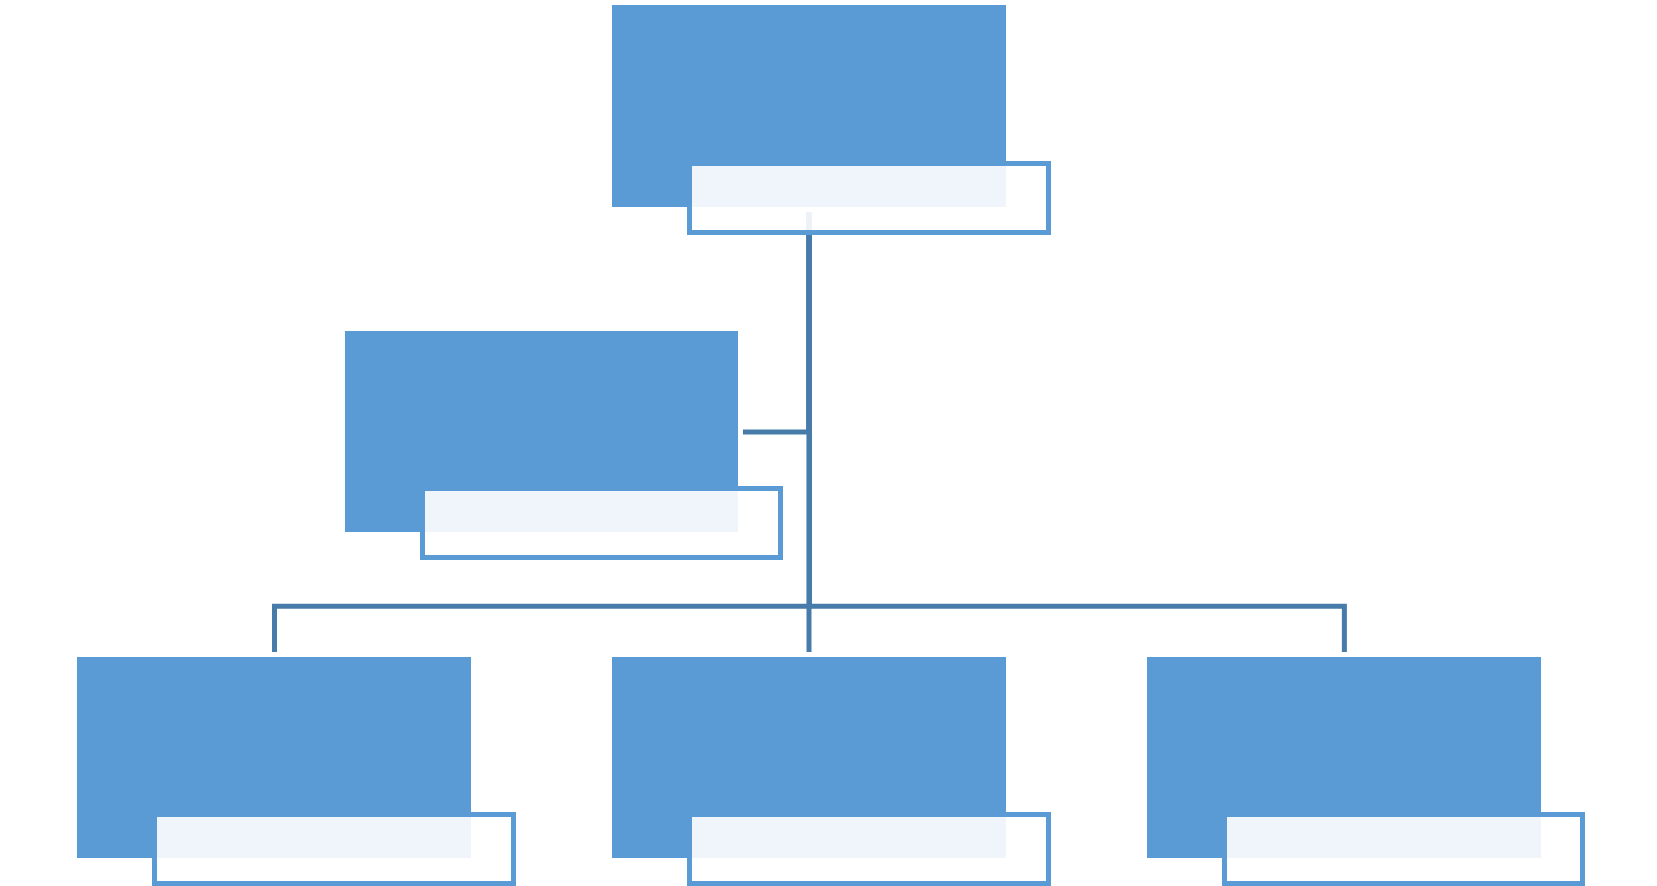
\includegraphics[width=0.75\textwidth]{figures/Fig1-1.png}
    \caption{全文组织结构图}\label{Fig1-1}
\end{figure}

各章主要内容简介如下：

第一章 绪论。介绍本文的研究背景与意义，综述大语言模型安全性、医疗AI安全性以及智能体测试技术的国内外研究现状，分析现有研究中存在的问题，阐述本文的研究内容和章节安排。

第二章 相关技术。介绍大语言模型的基本原理和架构，分析医疗大语言模型的特点和挑战，概述智能体技术的基本概念和发展历程，介绍大语言模型安全性评估的相关技术，为后续研究奠定理论基础。

第三章 MLSE框架设计。提出MLSE评估框架的整体架构，详细阐述框架的各个组成部分，包括测试用例生成模块、智能体执行模块、评估指标计算模块等。重点介绍模块化医疗智能体的设计方法，包括智能体的内部结构、工具调用机制、多智能体协作模式等。

第四章 智能体测试用例生成。详细阐述基于智能体的测试用例生成方法，包括医疗场景建模、测试策略设计、用例生成算法等。介绍如何利用智能体的规划和推理能力，自动生成覆盖多种安全风险类型的测试用例。

第五章 多维度安全性评估指标。建立面向医疗大语言模型的多维度安全性评估指标体系，包括准确性评估、安全性评估、可靠性评估、隐私保护评估等维度。详细介绍各指标的定义、计算方法和评估标准。

第六章 实验与分析。介绍MLSE框架的原型系统实现，包括系统架构、关键模块实现、界面设计等。设计全面的实验方案，对主流医疗大语言模型进行安全性评估，分析评估结果，验证框架的有效性。

第七章 总结与展望。总结全文的主要研究工作和创新点，分析研究的局限性，对未来研究方向进行展望。

